%%%%%%%%%%%%%%%%%%% Especificación:
\begin{frame}{Algoritmo:}{Propagación del tiempo vectorial.}
  \justifying
  \textbf{Notación:} Para, cualesquiera, dos vectores $Vc_1$
  y $Vc_2$ del tamaño $n$. Tenemos que
  \begin{itemize}
  \item[$\blacktriangleright$] $Vc_1 \leq Vc2 =_{def.}
    \left(\forall_{k \in \{1, \dotsm, n\}} : Vc_1[k] \leq Vc_2[k]\right)$;
  \item[$\blacktriangleright$] $Vc_1 < Vc2 =_{def.}
    \left(Vc_1[k] \leq Vc_2[k]\right) \land  \left(Vc_1[k] \not= Vc_2[k]\right)$;
  \item[$\blacktriangleright$] $Vc_1 || Vc_2 =_{def} \neg (Vc_1 \leq Vc_2) \land
    \neg (Vc_2 \leq Vc_1)$.
  \end{itemize}
  \begin{figure}
    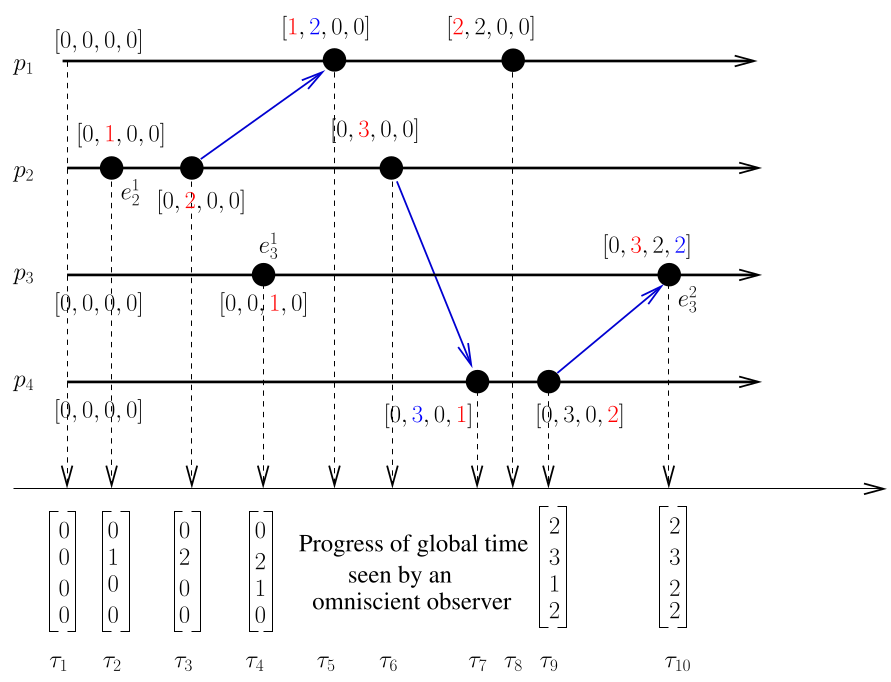
\includegraphics[height = 4.5cm]{./Imagenes/RelojVectorialCompuesto.png}
    \caption{Ejemplo de propagación en un reloj Vectorial.}
  \end{figure}
\end{frame}
